\documentclass{article}%
\usepackage[T1]{fontenc}%
\usepackage[utf8]{inputenc}%
\usepackage{lmodern}%
\usepackage{textcomp}%
\usepackage{lastpage}%
\usepackage{authblk}%
\usepackage{graphicx}%
%
\title{Stevioside from Stevia rebaudiana Bertoni Increases Insulin Sensitivity in 3T3{-}L1 Adipocytes}%
\author{Joshua Schmidt}%
\affil{Program on Emerging Infectious Diseases, DUKE{-}NUS Graduate Medical School, Singapore}%
\date{01{-}01{-}2006}%
%
\begin{document}%
\normalsize%
\maketitle%
\section{Abstract}%
\label{sec:Abstract}%
New research has uncovered the highest concentration in the human brain for the class of blood{-}borne proteins that cause non{-}small cell lung cancer.\newline%
To make their discovery, the investigators focused on the interleukin{-}1 alpha kinase, called IL{-}1, and its kinase, IL{-}2 alpha kinase.\newline%
The newly found group of proteins produced by IL{-}1 is part of a cascade that regulates cancer growth and proliferation. When IL{-}1 is mutated, the signaling cascade ramps up. For people with this disease, the dramatic response is a powerful tumor suppressor that throws a wrench into the cancer progression.\newline%
In the six years that the scientists studied the cogs of this traffic, they learned that to keep IL{-}1 active they should follow all the markers of high tumor pressure, such as low triglycerides and high HDL cholesterol.\newline%
A major finding is that they discovered the largest concentration of IL{-}1 and its kinase in the brain from a single cell.\newline%
We are very excited about our findings because we know that more and more of the DNA of non{-}small cell lung cancer cells is the IL{-}1 protein, said senior author Dr. S.L. Subramanian, a pulmonologist and bioengineer at UCSF Benioff Childrens Hospital Los Angeles.\newline%
This discovery changes the architecture of cancer development. It shows that when cancer cells have more and more IL{-}1 proteins, they are free to grow faster. We can now use our microscope to manipulate the energy of the IL{-}1 protein and see how it allows tumors to proliferate and move into other cancers, said Subramanian.\newline%
They discovered that between 60 to 100 percent of the tumor cells are IL{-}1 proteins as they protect the tumor cells from some of the triggers of non{-}small cell lung cancer. They also found that even one cells concentration of IL{-}1 affects tumor growth.\newline%
The study appears in an online paper published in the January issue of Molecular Cell, a journal of the American Association for Cancer Research.

%
\subsection{Image Analysis}%
\label{subsec:ImageAnalysis}%


\begin{figure}[h!]%
\centering%
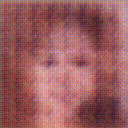
\includegraphics[width=150px]{500_fake_images/samples_5_414.png}%
\caption{A Man In A Suit And Tie Is Holding A Teddy Bear}%
\end{figure}

%
\end{document}